\documentclass{article}
\usepackage{amsmath}
\usepackage[]{algorithm2e}
\usepackage[a4paper, total={5.8in, 8in}]{geometry}
\usepackage{float}
\usepackage{url}
\usepackage{graphicx}
\usepackage{makecell}


\begin{document}
\title{\textbf{FYS4150/FYS3150 - Project 5}}
\author{Ingvild Bergsbak, Oliver Hebnes and Erlend Ousdal}
\date{October 24, 2018}


\maketitle
\begin{figure}[H]
  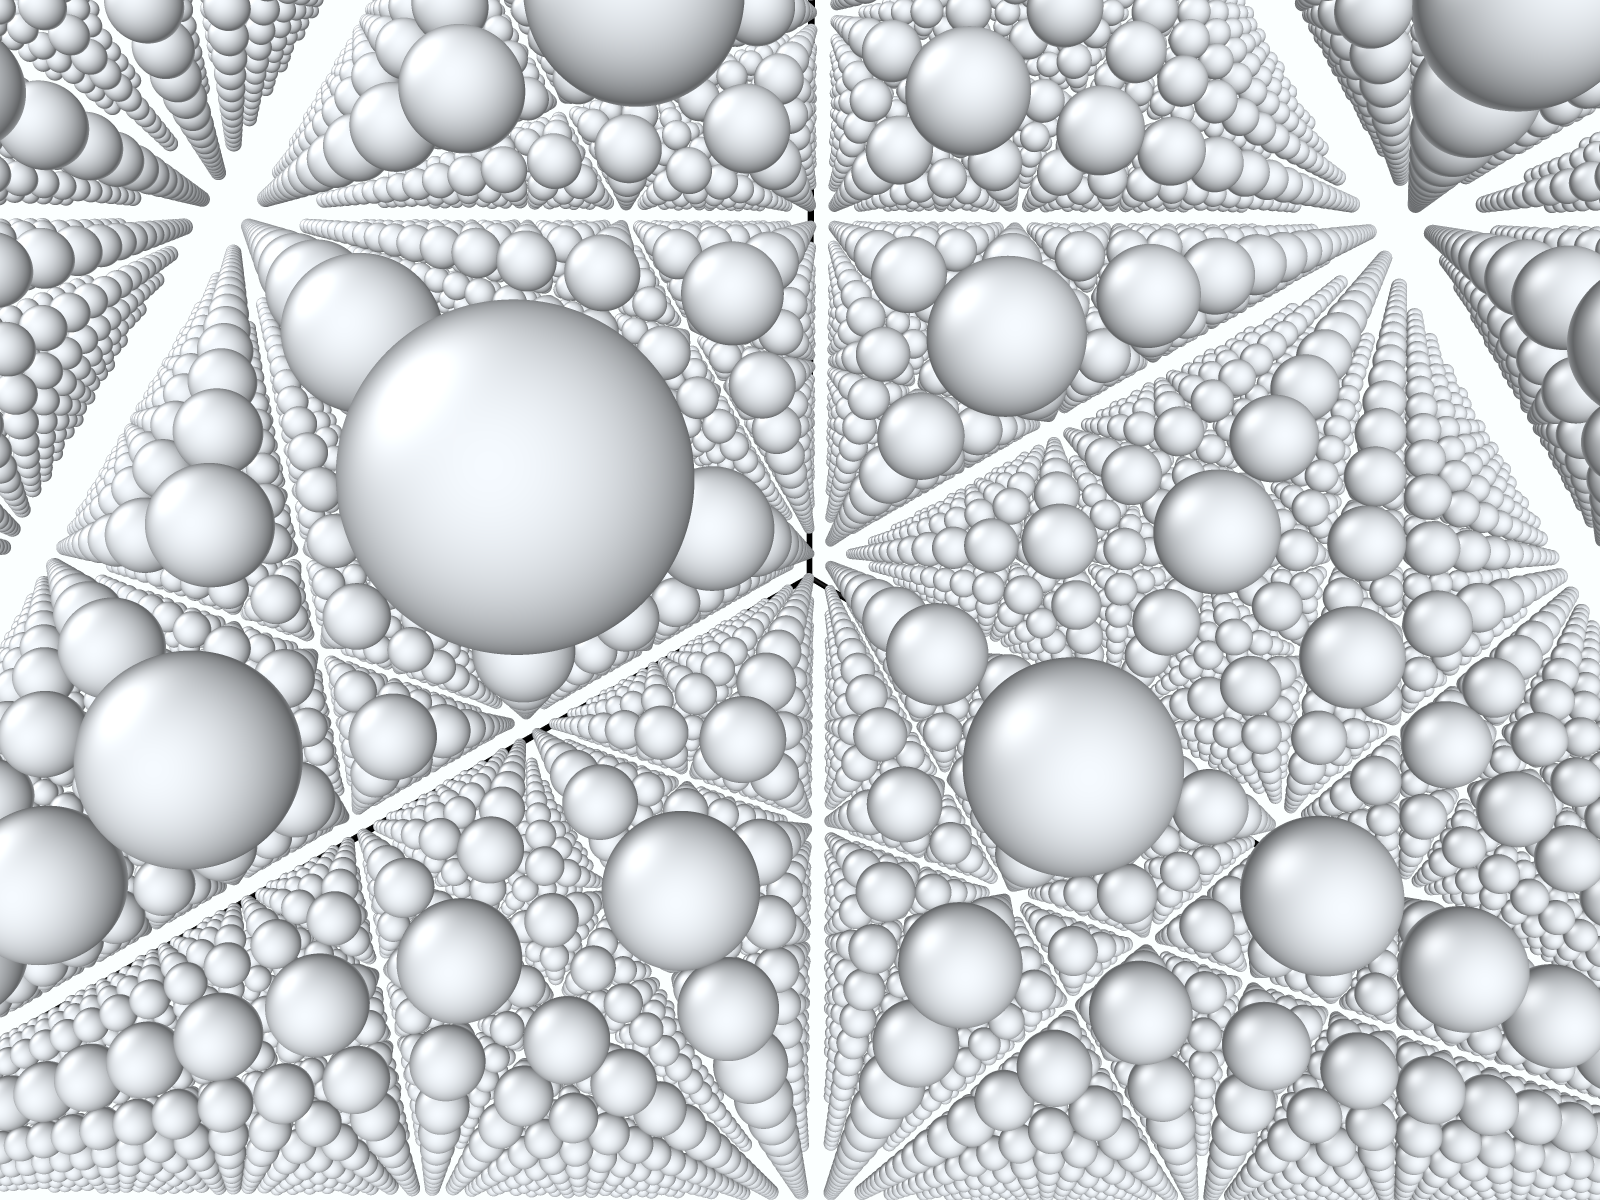
\includegraphics[scale=0.25]{plots/fcc_lattice_frontpage.png}
  \label{}
  \centering
\end{figure}

\newpage
\begin{abstract}
\end{abstract}
\section{Introduction}


\begin{figure}[h]
\begin{picture}(32,15)
\setlength{\unitlength}{0.14in} % selecting unit length \centering % used for centering Figure \begin{picture}(32,15) % picture environment with the size (dimensions)
\put(13,-4){\framebox(9,4){\thead{Initialize temperature, \\ number of unit cells, \\lattice constant and \\timestep}}}
\put(17,-4){\vector(0,-1){3}}
\put(13.5,-10){\framebox(8,3){\thead{Create FCC lattice \\ based on initial \\ conditions}}}
\put(17,-10){\vector(0,-1){3}}
\put(13.5,-16){\framebox(8,3){\thead{Remove total \\ momentum}}}
\put(17,-16){\vector(0,-1){4}}
\put(14,-22){\framebox(7,2){\thead{$t<$final time?}}}
\put(21,-21){\vector(1,0){4}}
\put(22, -20.5){\makebox{\thead{YES}}}
\put(25,-23){\framebox(18,4){\thead[l]{\, Sample\\ \, Calculate forces from Lennard-Jones potential \\ \, Apply periodic boundary conditions \\ \, $t+=dt$}}}
\put(28, -19){\line(0, 1){1}}
\put(28, -18){\vector(-1, 0){11}}
\put(17,-22){\vector(0,-1){3}}
\put(17.5, -23.75){\makebox{\thead{NO}}}
\put(15.25,-26.75){\framebox(3.75,1.75){\thead{End}}}

\end{picture}
\end{figure}
\vskip10cm


\section{Theoretical Methods and Thechnicalities}
\subsection{Molecular Dynamics}
Molecular dynamics is a very useful method for predicting the movement of molecules or atoms in relation to each other. It uses the Coloumb forces between the molecules and numerical integration to calculate the movement of the particles. Modelling a solid, for example, this method produces a prediction of the most likely lattice configuration.

\subsection{Periodic Boundary Conditions}
This far we have simply let the particles move with their initial velocity with no restrictions as if it was a dense gas expanding in a vacuum. However, this is not the scenario we would like to study. We want to look at a part of an infinite lattice, and to do so we need to implement periodic boundary conditions (PBC). Obviously, we cannot model an infinite lattice, but we model a small part, for instance a few unit cells, and make the assumption that the system consists of repeating units identical to the one we are looking at. In this case, PBC mean that a particle that moves outside of our defined "box", instead of continuing to move away from the box, it moves to the opposite side of the box as if it enters the box from an adjacent, identical box. In addition, the PBC need to compensate for the fact that the shortest distance between particles might be between different cells, not necessarily between particles in the same cell. To implement these conditions we added a few restrictions to the position and the distance between atoms, and the algorithm for the $x$ direction is shown below.

\begin{algorithm}[h]
\For{$atom_i$}{
	\If{rx $<$ -0.5size}{
		rx = rx + size\;
	}
	\If{rx $\geq$ 0.5size}{
		rx = rx-size\;
	}
	\For{$atom_j$}{
		\If{$atom_i$ $\neq$ $atom_j$}{
			dx = rx$_j$-rx$_i$\;
			\If{dx $>$ 0.5size}{
				dx = dx - size\;
			}
			\If{dx $\leq$ -0.5size}{
				dx = dx + size\;
			}
		}
	}
}
\end{algorithm}
To implement the PBC for three dimensions, the algorithm simply needs to be repeated for the $y$ and $z$ directions. These conditions will make sure the particles stay within the constant volume of our box.


\subsection{Maxwell-Boltzmann Distribution and Mean Velocity}
From statistical mechanics we know that the mean velocity of a particle depends on the temperature and can be calculated from the Boltzmann distribution for a particle with energy $E=\frac{1}{2}mv^2$ where $v=|\vec{v}|$. The most likely velocity is zero, but because our number of particles is far less than the number of possible velocities, the distributions of velocities will not follow the statistical distribution, and the sum of velocities for all the particles will not equal zero.



\subsection{The FCC-lattice}

Solid argon is most stable as a face-centered cubic lattice, where each unit cell contains four atoms. The lattice constant, which is the length of the side in the cubic unit cell, is $b=5.26$ Angstrom. The local coordinates are
\begin{align*}
	\vec{r_1} &= (0,0,0)\\
	\vec{r_2} &= (b/2,b/2,0)\\
	\vec{r_3} &= (0,b/2,b/2)\\
	\vec{r_4} &= (b/2,0,b/2)
\end{align*}
This way we can expand it into a three dimensional unit cell, where the origin of the system is located as
\begin{align*}
	\vec{R_{i,j,k}}=(i,j,k)
\end{align*}
where $i=0,1,...,N_x-1$, $j=0,1,...,N_y-1$, $k=0,1,...,N_z-1$.
\subsection{The Lennard Jones potential}

To calculate the force between two atoms we use the Lennard-Jones potential
\begin{align}
	U(r_{ij})=4\epsilon\Big[\Big(\frac{\sigma}{r_{ij}}\Big)^{12}-\Big(\frac{\sigma}{r_{ij}}\Big)^{6}\Big]
\end{align}

where $r_{ij}=|\vec{r_j}-\vec{r_i}|$ is the distance from atom $j$ to atom $i$, $\epsilon$ is the depth of the potential well and $\sigma$ is the distance where the potential is zero. The units that the system is using are

The definition of force is the negative derivative of the potential.
$$\mathbf{F}=-\nabla \mathbf{U}$$
where $\nabla$ is the Laplace operator.
The force is calculated by deriving the Lennard Jones potential. The force along the $x$-axis is

where $r_{ij}=|\vec{r_j}-\vec{r_i}|$ is the distance from atom $j$ to atom $i$, $\epsilon$ is the depth of the potential well and $\sigma$ is the distance at which the potential is zero.

\begin{align}
	F_x(r_{ij}) = - \frac{dU(r_{ij})}{dr_{ij}}\frac{dr_{ij}}{dx_{ij}}
	\label{forcex}
\end{align}
where the derivative of the potential is
\begin{align}
	\frac{dU}{dr_{ij}}=-12\frac{\sigma^{12}}{r_{ij}^{13}} + 6 \frac{\sigma^6}{r_{ij}^7}
\end{align}
and the derivative of the distance vector is
\begin{align}
	\frac{dr_{ij}}{dx_{ij}}&=\frac{d}{dx_{ij}}\sqrt{(x_j-x_i)^2+(y_j-y_i)^2+(z_j-z_i)^2}.
\end{align}
where $x_{ij}=x_j-x_i$ is the distance between atom $i$ and atom $j$ in $x$-direction.
\begin{align}
	\frac{dr_{ij}}{dx_{ij}}&=\frac{1}{r_{ij}}x_{ij}.
\end{align}
Inserting into equation \ref{forcex} will result in
\begin{align}
	F_x(r_{ij})= \epsilon \Big[48\frac{\sigma^{12}}{r_{ij}^{13}} - 24 \frac{\sigma^6}{r_{ij}^7}\Big]\frac{1}{r_{ij}}x_{ij}
\end{align}
The calculation of force is analogous in the $y$ and $z$ direction.


\subsection{Temperature}
The temperature is determined by the equipartition theorem
$$\langle E_k\rangle=\frac{3}{2}NkT$$
where $\langle E_k\rangle$ is the mean kinetic energy of the system, $N$ is the number of particles in the system, $k$ is Boltzmann's constant and $T$ is the temperature. As the system develops over time, the kinetic energy changes, leading to changes in the temperature of the system. The development of the temperature is kept track of by calculating the kinetic energy for each time step and using the equipartition theorem to find the temperature.


\subsection{Diffusion}
The diffusion constant of the system can be used to find the melting temperature. The constant is determined from the Einstein relation and its relation to the mean square displacement, $\langle r^2(t)\rangle$, is
$$\langle r^2(t)\rangle = 6Dt$$
where $D$ is the diffusion constant and $t$ is time. The mean square displacement is the average distance the particles of the system has traveled after a time $t$ and is defined as
$$\mathbf{r}_i^2(t)=(\mathbf{r}_i(t)-\mathbf{r}_i(0))^2$$
where $\mathbf{r}_i(t)$ is the position after a time $t$ and $\mathbf{r}_i(0)$ is the initial position of particle $i$. The diffusion constant is temperature dependent and describes how easily particles move in a system at a given temperature. Particles in a solid diffuses much slower than in liquid and gaseous phases, and the diffusion constant will be much smaller for temperatures at which the system is in the solid state than for temperatures above the melting point. Calculating the diffusion constant as a function of the temperature will therefore show a dramatic change around the melting point of the system and .


\subsection{Units of the system}

The SI-units are heavy to deal with on atomic level, and thus we chose to rescale them. Lattice size is usually measured in Angstrom, and mass is usually measured in atomic mass.
\begin{align}
	1 \textnormal{ unit of mass} &= 1 \textnormal{a.m.u} = 1.661\cdot 10^{-27}\, \textnormal{kg}\\
	1 \textnormal{ unit of length} &= 1 \textnormal{\AA} = 1.0\cdot 10^{-10}\, \textnormal{m}\\
	1 \textnormal{ unit of energy} &= 1.651\cdot 10^{-21}\,\textnormal{J}\\
	1 \textnormal{ unit of temperature} &= 119.735\,\textnormal{K}\\
	1 \textnormal{ unit of time} &= 1.00224\cdot 10^{-13}\, \textnormal{s}
\end{align}
From this we can calculate the Boltzmann constant as
\begin{align}
	K_B &= 1.38\cdot 10^{-23} \textnormal{m}^2\textnormal{kg}\textnormal{ s}^{-2}\textnormal{K}^{-1}\\
	&= 1.38\cdot 10^{-23} \cdot \frac{\textnormal{(unit of length)}^{-2}\cdot\textnormal{(unit of mass)}^{-1}}{\textnormal{(unit of time)}^{-2}\cdot\textnormal{(unit of temperature)}^{-1}}\\
	K_B &=1
\end{align}
Thus, $\frac{\epsilon}{k_B}=119.8K \textnormal{(unit of temperature)}^{-1}=1$ and $\sigma = 3.405 \textnormal{Å}\textnormal{ (unit of length)}^{-1} = 3.405$.

Similarly, it is possible to calculate the units of the force and the pressure;
\begin{align}
	\textnormal{1 unit of force} &= \textnormal{(unit of mass)}\cdot\frac{\textnormal{(unit of length)}}{\textnormal{(unit of time)}^2}\\
	 &= k_B \cdot \textnormal{(unit of temperature)}\cdot\textnormal{(unit of length)}\\
	\textnormal{1 unit of pressure} &=k_B \frac{\textnormal{(unit of temperature)}}{\textnormal{(unit of length)}^3}
\end{align}


\section{Results and Discussion}





\section{Conclusion}


\section{Appendix}
Link to the GitHub repository:\\

https://github.com/ohebbi/compphys.git

\begin{thebibliography}{}
\bibitem{termoboka}
Schroeder, Daniel V., \textit{An Introduction to Thermal Physics},Pearson, 2014\\
\end{thebibliography}

\end{document}
